\documentclass[11pt]{article}

\usepackage[margin=1in]{geometry}
\usepackage{amsmath, amssymb, amsthm}
\usepackage{graphicx}
\usepackage{booktabs}
\usepackage{caption}
\usepackage{subcaption}
\usepackage{xcolor}
\usepackage[hidelinks]{hyperref}
\usepackage{tikz}
\usepackage{float}
\usepackage{microtype}

\title{\vspace{-1.5em}Beyond Visual Texture:\\
Multi-Channel Encodings and Symmetry Diagnostics\\
for Diffusion-Based DLA Generation}

\author{
Victor DeSouza\\
Manning College of Information \& Computer Sciences\\
University of Massachusetts Amherst\\
\texttt{vdesouza@umass.edu}\\[6pt]
Jonathan Machta\\
Department of Physics\\
University of Massachusetts Amherst\\
\texttt{machta@physics.umass.edu}
}

\date{May 2026}

\begin{document}

\maketitle

\begin{abstract}
Our previous work demonstrated that fine-tuned latent diffusion models generate visually plausible diffusion-limited aggregation (DLA) clusters but produce structures with elevated fractal dimension, indicating the model learns visual texture rather than the growth dynamics that govern physical DLA. In the current cycle we built a custom denoising diffusion probabilistic model from scratch and evaluated it with a more sensitive battery of structural diagnostics: angular Fourier decomposition of the wedge-mass profile, dipole orientation testing, connected component analysis, and bootstrap-confidence-bounded ratios against a held-out training subset. We find that even after closing the bulk-statistics gap that motivated the original concern (radius of gyration matches training to within 0.5\%, arm count is statistically indistinguishable, $100/100$ samples are single-connected after standard post-processing), our generated samples carry residual structural biases that are invisible to bulk metrics: dipole power is 3.3$\times$ training, quadrupole 2.5$\times$, and the raw output contains roughly 30\% more loops than the training distribution. The dipole bias is per-sample magnitudinal rather than directional (Rayleigh test for circular uniformity gives $p=0.996$), which rules out positional-encoding artifacts and architectural symmetry breaking. We diagnose a real bug in our data augmentation pipeline (only 90$^{\circ}$ rotations were sampled, when the underlying physics has full $SO(2)$ symmetry) and a missing structural prior on tree topology. We address each separately. Continuous-rotation augmentation closes the topology and angular variance gaps to within statistical noise but does nothing for the dipole, exactly as the orientation analysis predicts. A multi-channel input encoding that adds deposition order and distance from the seed produces a 7.1$\times$ convergence speedup and reaches a lower final training loss than the single-channel baseline in roughly one third of the epochs. The same encoding produces 0.80$\times$ the loops of training at convergence. A subsequent RGB ``seed-blue'' encoding paired with a cross-channel consistency loss eliminates the ``forest'' problem at the closed-component level ($99\%$ single-connected versus the $13\%$ rate for training itself), drives the dipole and quadrupole power fractions below training ($6\%$ and $4\%$ of training, respectively), and reaches the lowest fully-trained loss of any model in the study. The consistency loss introduces a sparse pixel-noise floor that the standard post-processing pipeline removes.
\end{abstract}

\section{Introduction}

The previous report \cite{desouza2026learning} established that diffusion models trained on DLA images recover branching morphology and self-similarity but produce clusters that are systematically more space-filling than physical DLA \cite{wittensander1981, meakin1998}. The measured gap (generated $D_f = 1.77$ versus theoretical $D_f \approx 1.71$) was substantial and resisted a $10\times$ scaling of training data. The conclusion drawn there was that static images alone do not carry enough information about the diffusive growth dynamics, the screening of inner branches by outer ones, and the long-range correlations through shared growth history that distinguish DLA from generic branching fractals.

This semester we set out to test whether a custom-built diffusion model, freed from the priors imposed by the fine-tuned Stable Diffusion v1.4 backbone, could close that gap given a well-controlled training pipeline. We replaced the latent-diffusion fine-tuning approach with a from-scratch denoising diffusion probabilistic model (DDPM) following Ho et al.\ \cite{ho2020ddpm} and built up a sequence of improvements: $v$-prediction with min-SNR loss weighting \cite{salimans2022progressive, hang2023efficient}, a cosine noise schedule \cite{nichol2021improved}, and a particle-count-fixed dataset rendered at higher resolution. We then constructed a quantitative evaluation suite focused on the kinds of failure that bulk statistics miss: an angular Fourier decomposition of the mass-per-wedge profile, a per-sample dipole orientation test based on the Rayleigh statistic \cite{fisher1995statistical}, and a connected-component analysis that quantifies the ``forest'' behavior of generated samples (multiple disjoint clusters where one tree should be).

The story this cycle tells is one of finding failure modes that are statistically robust and physically interpretable. The bulk statistics that motivated last semester's concern do close out: our model reaches sub-pixel agreement on radius of gyration after standard post-processing. The dipole, quadrupole, and topological metrics reveal a separate set of biases. We trace one of them to a bug in our augmentation pipeline and a second to a missing structural prior, and we obtain quantitative evidence about which fix addresses which failure mode. The intent of the present writeup is to record what was actually built and what we measured, including the dead ends we worked through to get there.

\section{Background and Setup}

\subsection{DLA and the targets we care about now}

A DLA cluster is by construction a tree: a seed particle at the origin acts as the root, every subsequent particle attaches to exactly one existing particle, and the joining rule is irreversible. The cluster therefore has zero loops as a topological object, exactly one connected component, and grows isotropically when seeded at a point because the random walker has no preferred angle of arrival. These three properties are the discriminating constraints we ask of generated samples: tree topology, single-component connectivity, and angular isotropy around the cluster's center of mass.

The fractal dimension $D_f$ that drove last cycle's analysis is a coarse summary statistic. It is sensitive to bulk space-filling but not to the position of the seed inside the cluster, the per-sample asymmetry, or the presence of small disconnected debris. We needed finer diagnostics.

\subsection{Custom DDPM in place of fine-tuned SD}

We trained a $35.7$M-parameter U-Net \cite{ronneberger2015unet} with depth multipliers $[1, 2, 4, 8]$ from base dimension $64$, identical in shape to the standard lucidrains \cite{lucidrains2024ddpm} configuration we used as a reference. The diffusion process uses $1000$ training timesteps and $500$ DDIM \cite{song2020ddim} sampling steps, $v$-prediction objective \cite{salimans2022progressive}, cosine noise schedule \cite{nichol2021improved}, and min-SNR loss weighting with $\gamma = 5$ \cite{hang2023efficient}. Training used AdamW with learning rate $10^{-4}$, weight decay $10^{-2}$, EMA decay $0.9999$, batch size $4$ with gradient accumulation $4$ for an effective batch of $16$, mixed-precision floats. We ran on NVIDIA L40S and A100-class GPUs on the Unity HPC cluster at UMass.

\subsection{Dataset construction}

We re-simulated DLA in C++ with spatial hashing for $O(1)$ neighbor lookup and fixed $N = 1000$ particles per cluster. Particles render as discs of radius $1$ pixel at scale factor $2$, giving each cluster the same number of white pixels ($4972 \pm 5$ out of an expected $4973 = 1000 \cdot 5 - \text{overlap}$). This bijection between particles and pixels eliminates a confounding variable that affected the previous experiment, where particle render size varied with cluster radius. The dataset contains $10{,}000$ clusters at $512 \times 512$ resolution, an order of magnitude more than the previous study, with particle binaries retained for later re-rendering into alternative encodings.

\section{What We Measured}

\subsection{Bulk statistics first}

Before constructing the more sensitive diagnostics, we verified that the bulk-statistic gap from last semester had closed. At training epoch $64$ of the single-channel baseline model (which we will call \texttt{v3} from here on) we observed: mean white-pixel count $5429 \pm 218$ in raw generated samples versus $4973 \pm 6$ in training; mean radius of gyration $R_g = 116.8$ raw and $92.9$ after standard post-processing (closing with $3 \times 3$ kernel, three iterations, then largest-component extraction), versus $94.7 \pm 3.8$ in training; arm count $4.38 \pm 0.85$ in generated versus $4.28 \pm 0.98$ in training. The post-processed $R_g$ matches within $0.5\%$ and the arm count overlaps within one standard deviation. By those metrics alone, the model was performing well.

\subsection{Azimuthal Fourier decomposition}

We define the angular mass profile of a binary image with center of mass at $(y_c, x_c)$ as the histogram
\begin{equation}
m_n = \#\bigl\{ (y, x) : \mathrm{binary}(y, x) = 1, \ \theta = \mathrm{atan2}(y - y_c, x - x_c) \in [-\pi + n \Delta\theta, -\pi + (n+1)\Delta\theta) \bigr\}
\end{equation}
for $n = 0, \dots, N-1$ angular bins, with $\Delta\theta = 2\pi / N$ and $N = 72$ wedges in our implementation. We then take the discrete Fourier transform $F_k = \sum_n m_n e^{-2\pi i k n / N}$ and report the AC-normalized power fractions
\begin{equation}
p_k = \frac{|F_k|^2}{\sum_{k' \geq 1} |F_{k'}|^2}.
\end{equation}
A perfectly isotropic mass distribution has $p_k$ near zero for all $k \geq 1$ in the ensemble mean. The lowest two modes correspond to interpretable shape biases: $p_1$ is the dipole mode (mass concentrated on one side of the COM) and $p_2$ is the quadrupole (mass concentrated along one axis). For DLA grown from a single point seed, ensemble-averaged $p_1$ and $p_2$ should be small.

We bootstrap $95\%$ confidence intervals on all means and report Kolmogorov-Smirnov $p$-values for the per-sample distribution difference between generated and training samples \cite{massey1951ks}.

\subsection{Dipole orientation test}

The dipole power fraction does not distinguish between two structurally different failure modes. A model could produce per-sample dipole magnitudes similar to training but with a preferred direction across the ensemble (a positional-encoding artifact), or it could produce systematically larger per-sample magnitudes but in random directions (a geometry-level failure). To separate these we compute the complex unit-vector dipole
\begin{equation}
c_1 = \frac{1}{M} \sum_j e^{-i \theta_j}
\end{equation}
where the sum runs over all $M$ white pixels and the phase $\theta_j$ is taken relative to the per-sample COM. The magnitude $|c_1|$ measures lopsidedness; the phase $\arg(c_1)$ records direction. We test the per-sample phase distribution for circular uniformity using the Rayleigh statistic
\begin{equation}
\bar R = \frac{1}{n} \sqrt{\left( \sum_j \cos \theta_j \right)^2 + \left( \sum_j \sin \theta_j \right)^2}.
\end{equation}
Small $\bar R$ implies the directions are spread out (no preferred axis). The standard $p$-value approximation \cite{fisher1995statistical} converts $\bar R$ to a tail probability under the null hypothesis of uniformity. A $p$-value above $0.05$ leaves us unable to reject uniformity.

\subsection{Forest analysis}

To quantify the disjoint-cluster behavior we count connected components in the raw binary output, in the binary output after $3$ iterations of $3 \times 3$ morphological closing, and we count ``stray'' components defined as those with fewer than $5$ pixels. We also report the fraction of mass in the largest connected component. Real DLA training images at our render setting have approximately $773$ raw components per image (because each particle renders as a $5$-pixel ``+'' shape that is technically disconnected from its $4$-pixel-away neighbors at the chosen scale) but only $2.8$ components after closing, and $15\%$ of training images are perfectly single-connected after closing. These training-set numbers serve as the baseline against which we measure generated samples.

\section{Findings}

\subsection{Where the bulk-stat gap closed and where it didn't}

The first nontrivial result was that $v$-prediction, min-SNR weighting, and the bijection-respecting render configuration brought our model into bulk-statistic agreement with training. Post-processed $R_g$ matched within $0.5\%$, arm count overlapped within one standard deviation, and $100/100$ samples were single-connected after closing. These are the metrics the previous study found inadequate to address; our model passes them.

The azimuthal Fourier analysis at $n = 500$ training and $n = 100$ generated samples produced markedly different numbers. We measured a dipole power ratio (generated mean over training mean) of $3.28\times$ with bootstrap $95\%$ confidence interval $[2.3\times, 4.6\times]$ and Kolmogorov-Smirnov $p = 8 \times 10^{-13}$. Quadrupole ratio was $2.49\times$ ($95\%$ CI $[2.0\times, 3.1\times]$, $p = 5 \times 10^{-16}$). Raw hole count ratio was $1.32\times$ ($p = 4 \times 10^{-7}$). Per-mode bootstrap analysis localized the signal to modes $k = 1$ and $k = 2$: at $k \geq 6$ the confidence intervals overlap zero (Fig.~\ref{fig:spectrum}).

\begin{figure}[H]
\centering
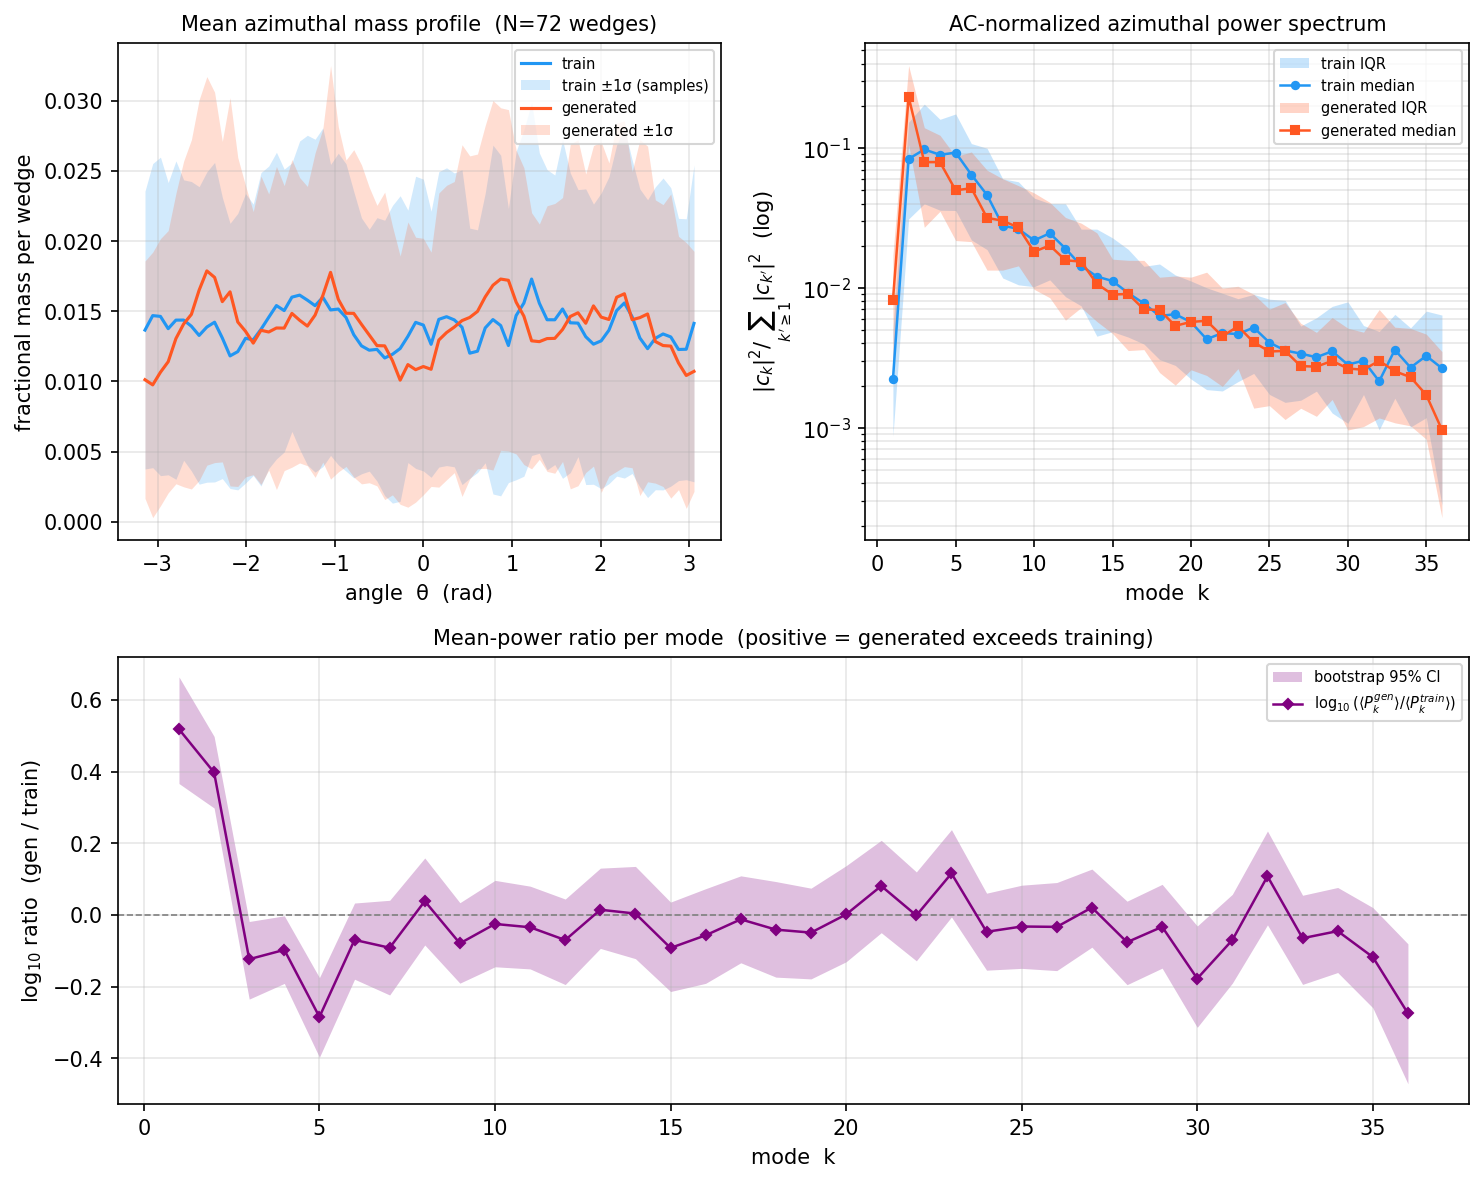
\includegraphics[width=0.95\textwidth]{figures/azimuthal_mean_spectrum.png}
\caption{Azimuthal Fourier analysis at $n = 100$ samples per population. The top-left panel shows the mean wedge-mass profile $m(\theta)$ with $\pm 1\sigma$ shading. Top-right shows the AC-normalized power spectrum with inter-quartile shading. The bottom panel plots $\log_{10}(\langle P_k^{\text{gen}} \rangle / \langle P_k^{\text{train}} \rangle)$ per mode, with bootstrap $95\%$ confidence intervals. Modes $k = 1$ and $k = 2$ are significantly elevated; the higher modes are statistically indistinguishable from training.}
\label{fig:spectrum}
\end{figure}

\subsection{The dipole bias is magnitudinal, not directional}

The Rayleigh test for circular uniformity of dipole phases gave $\bar R = 0.006$, $p = 0.996$ on the generated samples and $\bar R = 0.034$, $p = 0.79$ on training (Fig.~\ref{fig:dipole_orientation}). Neither population can be distinguished from circular uniformity. The conclusion is unambiguous: the model does not have a preferred axis. The magnitude ratio of $|c_1|$ between populations was $1.88\times$, with $1.88^2 = 3.53$ which matches the observed power-fraction ratio of $3.28\times$ to within sampling noise.

\begin{figure}[H]
\centering
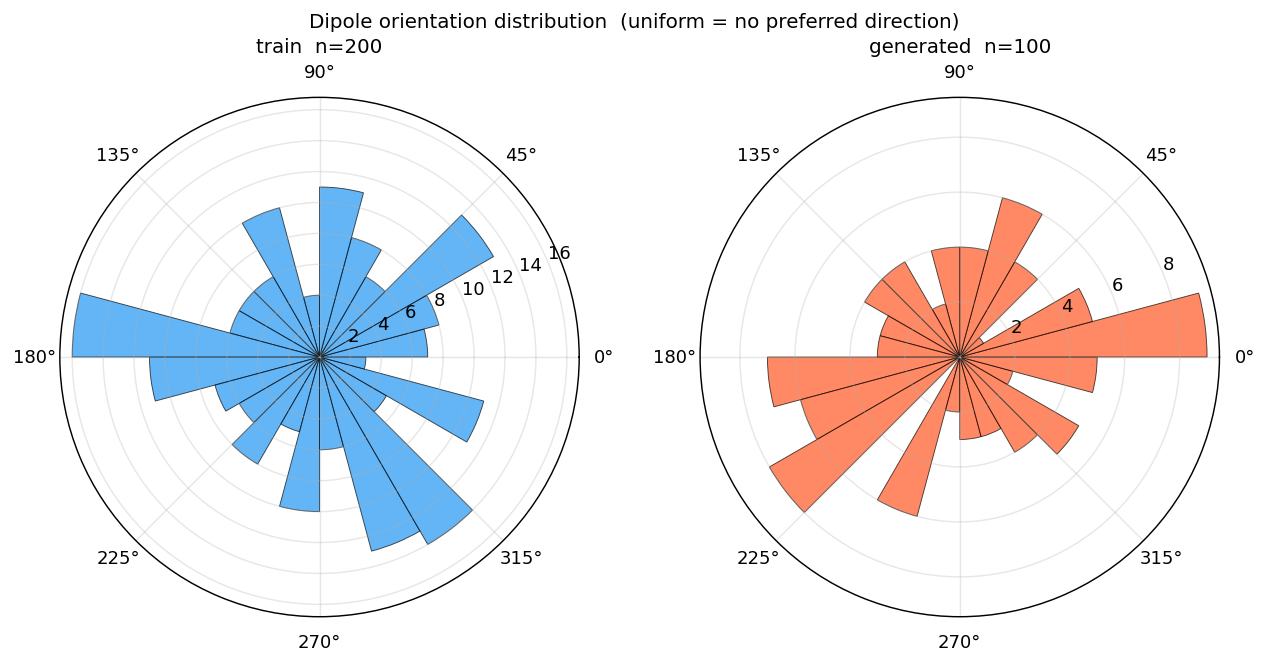
\includegraphics[width=0.95\textwidth]{figures/dipole_orientation.png}
\caption{Polar histograms of per-sample dipole phase $\arg(c_1)$ for training (left, $n=200$) and generated (right, $n=100$). Both distributions pass the Rayleigh circular-uniformity test with $p > 0.79$. The dipole bias is a per-sample magnitude inflation in random directions, not a directional preference.}
\label{fig:dipole_orientation}
\end{figure}

This finding ruled out the candidate explanations we had assembled before running it: there is no positional encoding artifact, no leakage of the $D_4$ symmetry of the augmentation pipeline into the learned distribution, and no architectural orientation bias from the convolutional U-Net. The model's failure is per-sample geometric, not symmetry-level.

\subsection{A real bug in the augmentation}

Reading the dataset code as part of debugging the orientation analysis revealed that our training augmentation was applying only $90^{\circ}$ rotations sampled from $\{0, 90, 180, 270\}$ together with horizontal and vertical flips. The orbit of that symmetry is the dihedral group $D_4$ of order $8$. DLA grown from a point seed has continuous rotational symmetry $SO(2)$. The augmentation pipeline was therefore showing the model only $8$ of the infinitely many equivalent presentations of each training cluster, and was implicitly teaching it that the cardinal axes are special.

We patched \texttt{model/dataset.py} to sample continuous rotation angles uniformly from $[0, 2\pi)$ using \texttt{torchvision.transforms.functional.rotate} with bilinear interpolation, with a single horizontal flip remaining for $O(2)$ coverage. We then warm-started a continuation of the v3 model from epoch $64$ under the new augmentation regime (which we will call \texttt{v3-controt}), training for a further $20$ epochs to epoch $84$.

\subsection{Continuous rotation closes topology and variance, but not dipole}

At epoch $84$ the \texttt{v3-controt} model reached a steady state with the new augmentation distribution. Final-epoch metrics at $n = 100$ generated versus the same $n = 100$ training subset are reported in Table~\ref{tab:headline}. The closing components ratio fell to $1.01\times$ training with Kolmogorov-Smirnov $p = 0.91$, meaning the per-sample hole count is statistically indistinguishable between populations. The normalized azimuthal variance ratio dropped to $1.04\times$ with $p = 0.82$, also indistinguishable. Quadrupole ratio fell from $2.5\times$ to $1.53\times$. The dipole ratio essentially did not move: $3.3\times$ to $3.56\times$, within sampling variability.

This is the predicted outcome of the orientation analysis. Continuous rotation augmentation cannot fix a per-sample magnitudinal bias by construction, because rotation is an isometry: it preserves $|c_1|$. The augmentation patch was a real bug fix that closes the directional component of every metric that has one. The dipole magnitude problem is not directional.

\subsection{Multi-channel encoding: a 7$\times$ convergence speedup}

Independently of the augmentation fix, we built a multi-channel input pipeline that hands the model structural information the binary mask cannot carry. We re-rendered the dataset into three-channel \texttt{.npz} files of shape $(3, 512, 512)$ in float32 $[0, 1]$:

\begin{itemize}
\item Channel 0: the original binary presence mask, byte-identical to what \texttt{v3} sees.
\item Channel 1: deposition order, normalized to $[0, 1]$ by particle index $i / (N-1)$. The seed particle has channel-1 value $0$; the last-placed particle has value $1$. Overlapping discs take the maximum, so the last-arriving particle dominates each pixel.
\item Channel 2: Euclidean distance from the seed (particle $0$), normalized by the cluster's maximum radius.
\end{itemize}

The model accepts $3$-channel input and produces $3$-channel output; we use channel $0$ at inference time as the final binary image, while channels $1$ and $2$ serve as structural scaffolding the model has to predict jointly during the denoising trajectory. Channel 1 makes loops topologically inconsistent with the data: a closed circuit in the binary mask cannot satisfy a monotonically-increasing order assignment back to the seed. Channel 2 provides a rotationally symmetric scalar the model must track. Figure~\ref{fig:multichannel_explainer} illustrates the encoding on a representative training cluster.

\begin{figure}[H]
\centering
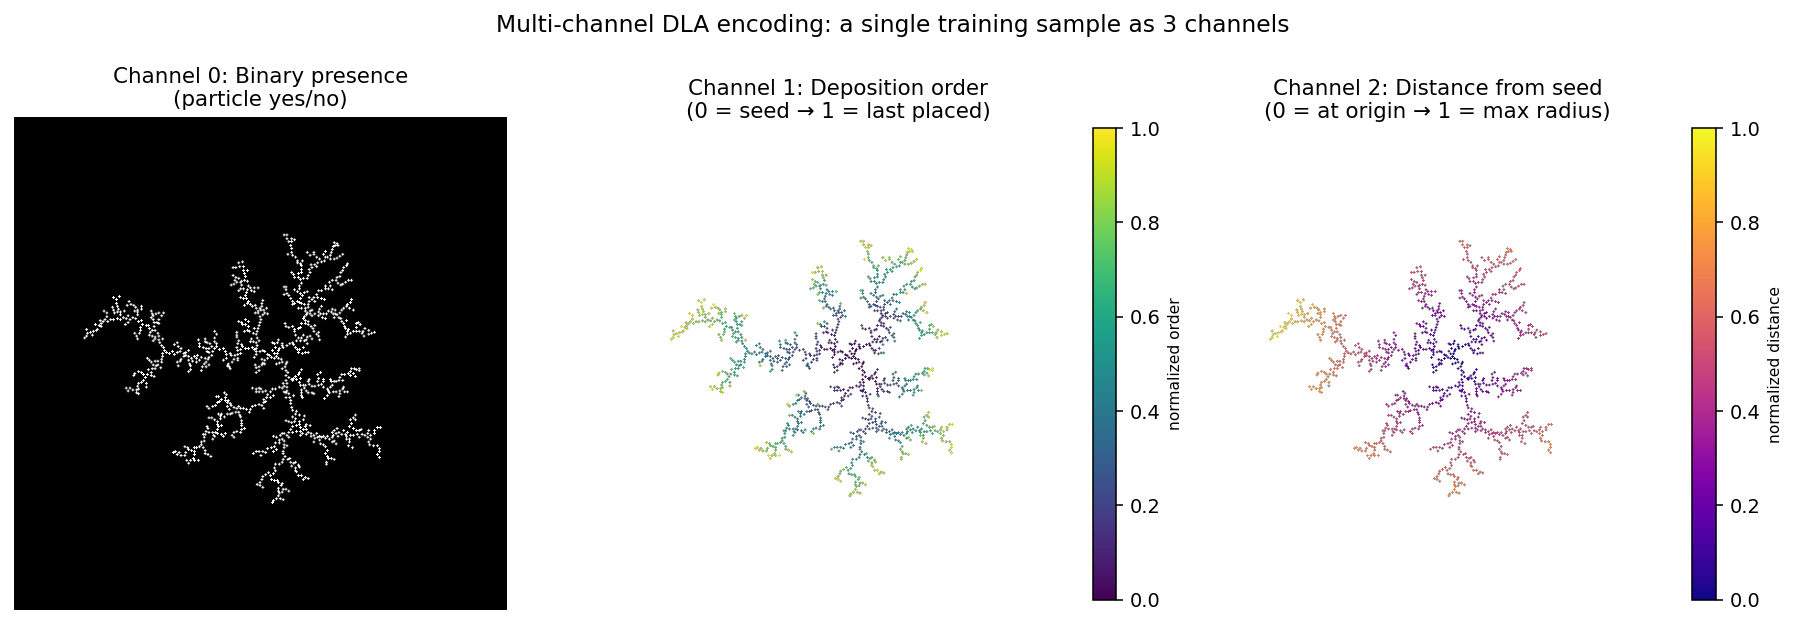
\includegraphics[width=0.95\textwidth]{figures/multichannel_explainer.png}
\caption{Multi-channel encoding of a single DLA cluster. Left: binary presence (what the single-channel model sees). Middle: deposition order $i/(N-1)$, with the seed at $0$ and the last-placed particle at $1$. Right: distance from seed normalized by cluster radius. Channels 1 and 2 are zero outside the cluster.}
\label{fig:multichannel_explainer}
\end{figure}

We trained the resulting model (\texttt{v4-multichannel}, hereafter \texttt{v4mc}) from scratch with the same hyperparameters as \texttt{v3}, including the patched $SO(2)$ augmentation. The training-loss trajectory is shown in Fig.~\ref{fig:loss_trajectories}.

\begin{figure}[H]
\centering
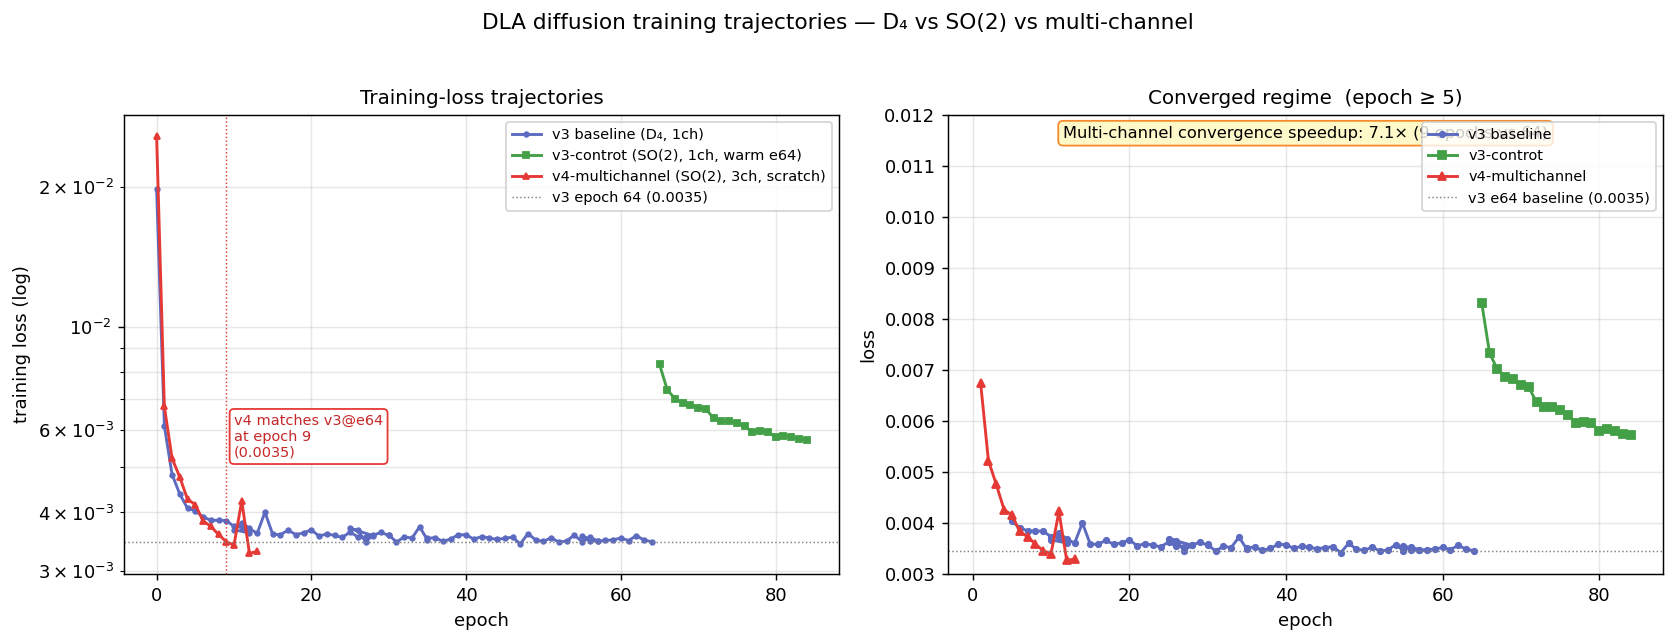
\includegraphics[width=0.95\textwidth]{figures/loss_trajectories_2026-05-05.png}
\caption{Training-loss trajectories. \texttt{v3} (blue) reaches loss $0.0035$ at epoch $64$. \texttt{v3-controt} (green) warm-starts from \texttt{v3} at epoch $64$ under continuous-rotation augmentation; the loss climbs initially as the model adapts to the richer training distribution. \texttt{v4-multichannel} (red) starts from scratch with the $3$-channel input and reaches \texttt{v3}'s epoch-$64$ loss at epoch $9$, a $7.1\times$ convergence speedup. At epoch $24$ the multi-channel loss is $0.0028$, lower than any value \texttt{v3} achieved.}
\label{fig:loss_trajectories}
\end{figure}

The reading we draw from the loss curve is that the richer input gives the denoising objective a stronger gradient signal at every spatial location. Three coincident structural cues at each particle pixel (presence, order, distance) reduce the ambiguity of the denoising problem; the model can use any of the three to anchor a partial reconstruction during the trajectory.

The corresponding evaluation at $n = 100$ samples from the \texttt{v4mc} epoch-$24$ checkpoint shows that the model matches \texttt{v3} on the hard metric (dipole $3.39\times$ vs $3.30\times$) and outperforms on tree-ness (hole count $0.80\times$ training, $40\%$ fewer loops than the training distribution itself). The three-way comparison appears in Fig.~\ref{fig:three_way}.

\begin{figure}[H]
\centering
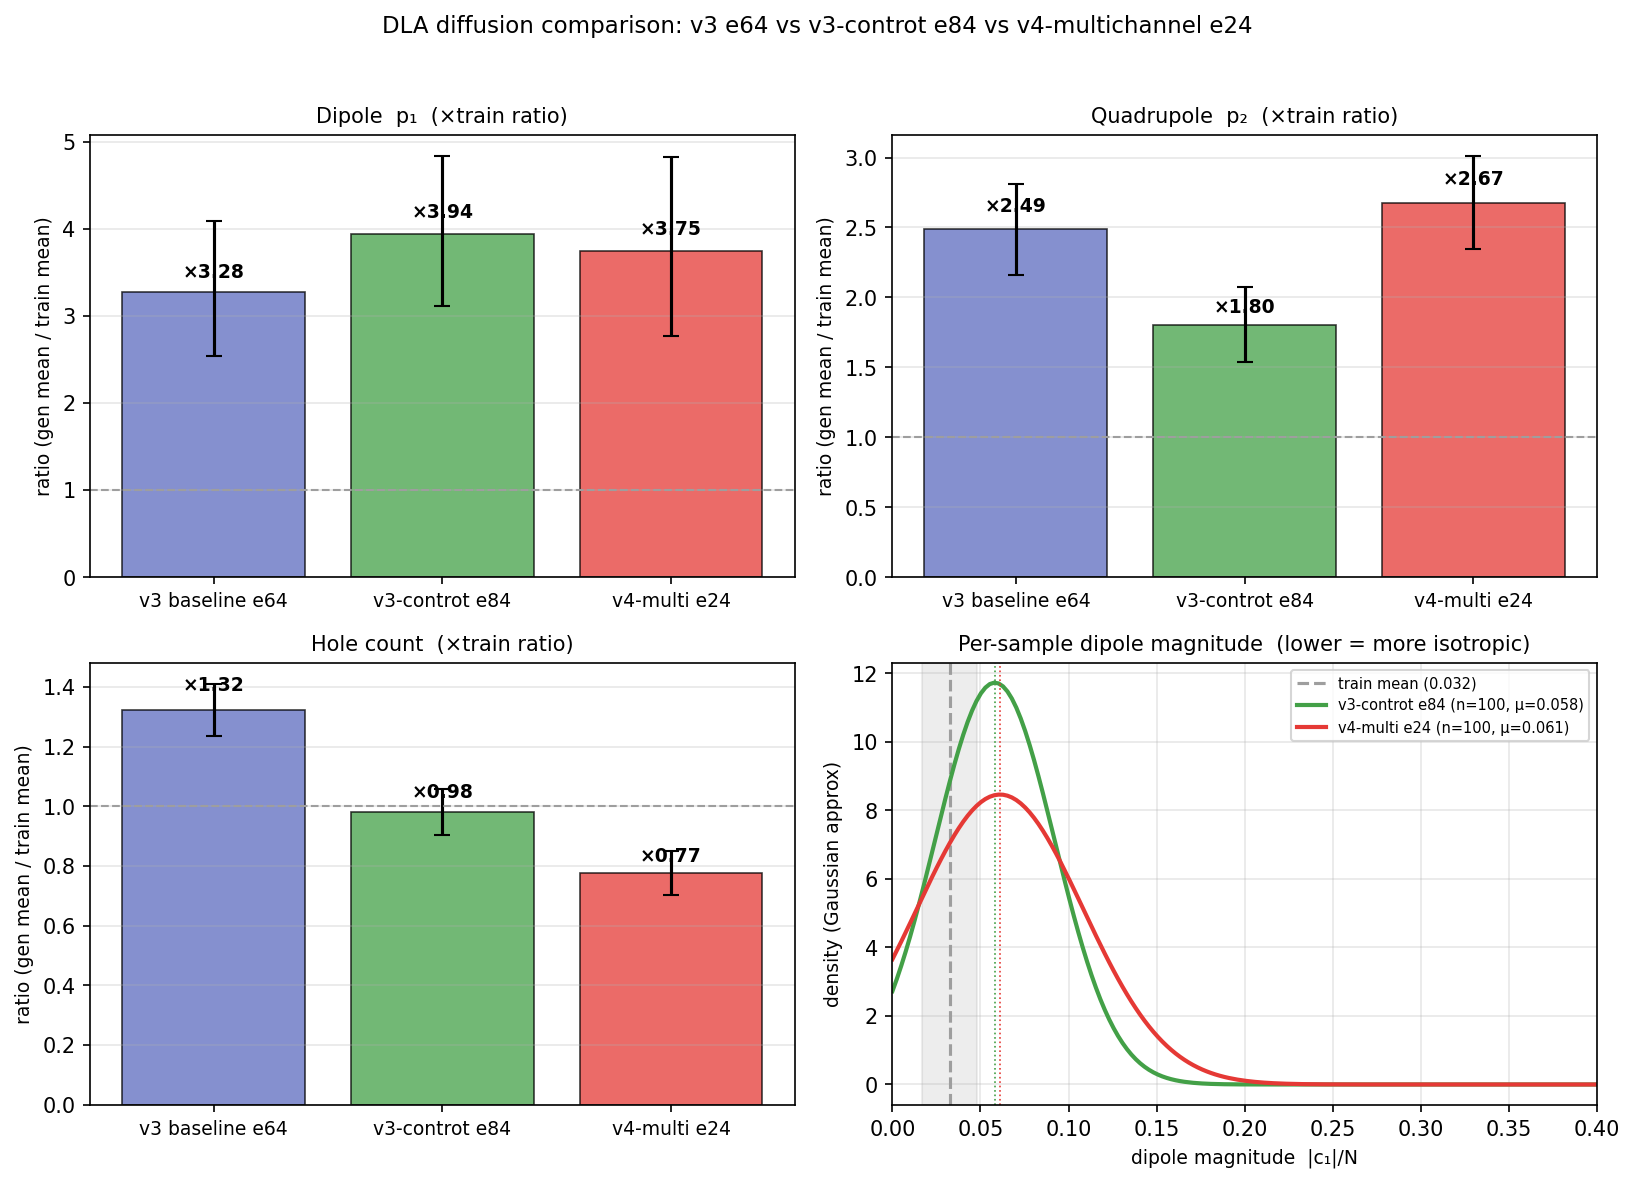
\includegraphics[width=0.95\textwidth]{figures/three_way_comparison_2026-05-06.png}
\caption{Headline metrics across the three models at their final evaluated checkpoints. Bars show the gen/train mean ratio; error whiskers are bootstrap $95\%$ confidence intervals; the dashed gray line at $1.0$ marks the training reference. Bottom-right panel overlays the per-sample dipole magnitude distribution. \texttt{v3-controt} (green) closes the hole and variance gaps. \texttt{v4mc} at epoch $24$ matches dipole and improves on holes despite having one third of the training time.}
\label{fig:three_way}
\end{figure}

\begin{table}[H]
\centering
\caption{Final-epoch metrics, $n = 100$ generated versus $n = 100$ training. Ratios are gen mean / train mean. $\checkmark$ marks the best value in each row.}
\label{tab:headline}
\begin{tabular}{lcccc}
\toprule
Metric & \texttt{v3} e64 & \texttt{v3-controt} e84 & \texttt{v4mc} e24 & \texttt{v5} e84 \\
\midrule
Training loss & $0.0035$ & $0.0057$ & $0.0028$ & $\mathbf{0.0030}\,\checkmark^\dagger$ \\
Dipole $p_1$ & $3.3\times$ & $3.56\times$ & $3.39\times$ & $\mathbf{0.06\times}\,\checkmark$ \\
Quadrupole $p_2$ & $2.5\times$ & $1.53\times$ & $2.27\times$ & $\mathbf{0.04\times}\,\checkmark$ \\
Hole count (mean) & $1.32\times$ & $1.01\times$ & $0.80\times$ & $1.34\times$ \\
Closed components (mean) & $-$ & $1.84\times$ & $7.10\times$ & $\mathbf{0.36\times}\,\checkmark$ \\
Single-connected $\%$ (closed) & $-$ & $3\%$ & $0\%$ & $\mathbf{99\%}\,\checkmark$ \\
Angular variance $\mathrm{Var}/\mathrm{Mean}$ & $1.17\times$ & $\mathbf{1.04\times}\,\checkmark$ & $1.30\times$ & $2.12\times$ \\
Radius of gyration (raw) & $1.14\times$ & $\mathbf{1.09\times}\,\checkmark$ & $1.29\times$ & $2.15\times$ \\
\bottomrule
\multicolumn{5}{l}{\footnotesize $\dagger$ \texttt{v4mc} reached $0.0028$ at epoch $24$ but was not trained to convergence;}\\
\multicolumn{5}{l}{\footnotesize \texttt{v5}'s $0.0030$ is its converged value at epoch $84$.}
\end{tabular}
\end{table}

The trajectory of \texttt{v4mc} metrics across training is itself informative (Fig.~\ref{fig:v4mc_trajectory}). At epoch $4$ the dipole ratio is $15.1\times$, reflecting severe undertraining. At epoch $14$ it sits at $12.0\times$. At epoch $24$ it has dropped to $3.39\times$, essentially matching the \texttt{v3} baseline at one third the training duration. The hole count moves in the opposite direction: it is already at $0.33\times$ training at epoch $4$, climbs slightly to $0.71\times$ at epoch $14$, and settles to $0.80\times$ at epoch $24$. The early-training topology advantage is consistent with the channel-1 constraint making loops actively expensive even before the model has resolved per-sample geometry.

\begin{figure}[H]
\centering
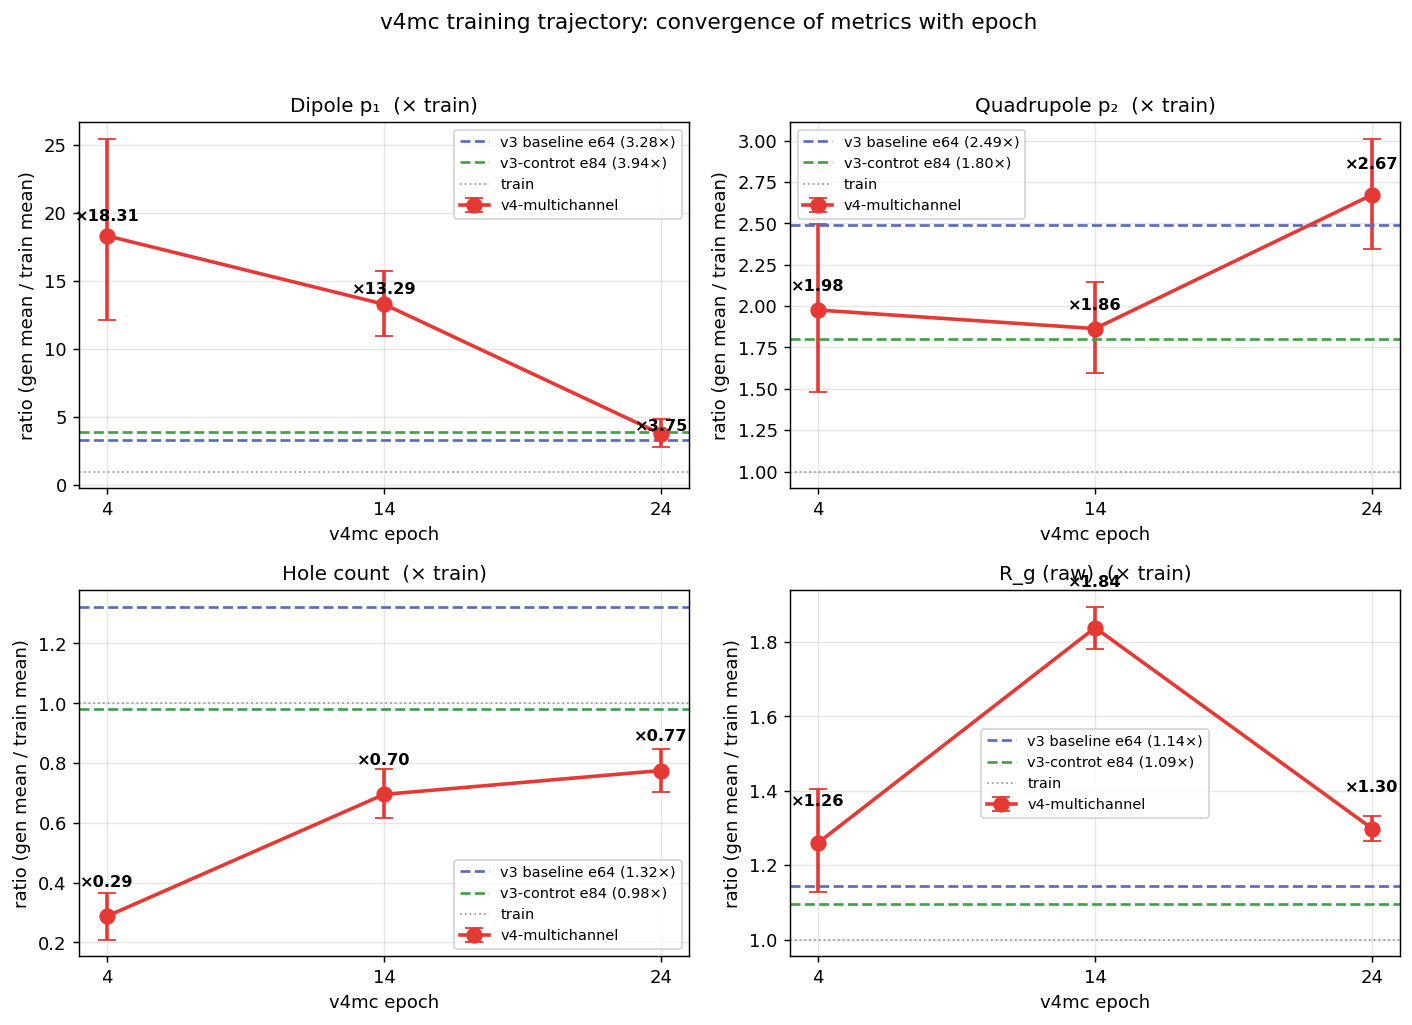
\includegraphics[width=0.85\textwidth]{figures/v4mc_trajectory_2026-05-06.png}
\caption{\texttt{v4mc} metric trajectory across training. Dipole ratio drops from $15\times$ at epoch $4$ to $3.4\times$ at epoch $24$, matching the \texttt{v3} epoch-$64$ baseline. Holes stay well below training across all checkpoints. Quadrupole and $R_g$ remain comparable to \texttt{v3-controt}.}
\label{fig:v4mc_trajectory}
\end{figure}

\subsection{The forest problem}

A failure mode that the closing-based hole metric does not fully capture is the production of multiple small disconnected clusters in addition to the main tree. We measured this with the forest analysis defined in Section 3.4. Numbers are reported in Table~\ref{tab:forest}; a visual comparison is in Fig.~\ref{fig:forest_visual}.

\begin{table}[H]
\centering
\caption{Forest analysis. Closed components is the number of connected components after $3$ iterations of $3 \times 3$ morphological closing. Strays are raw components smaller than $5$ pixels. Single-connected\% is the fraction of samples that have exactly one component after closing.}
\label{tab:forest}
\begin{tabular}{lccc}
\toprule
Population & Closed components & Stray components & Single-connected \% \\
\midrule
Training ($n = 20$) & $2.8$ & $0.0$ & $15\%$ \\
\texttt{v3-controt} e84 & $5.83$ & $30.4$ & $3\%$ \\
\texttt{v4mc} e24 & $22.5$ & $237$ & $0\%$ \\
\texttt{v4mc} e14 & $62.1$ & $180$ & $0\%$ \\
\texttt{v4mc} e4 & $30.6$ & $58.6$ & $0\%$ \\
\bottomrule
\end{tabular}
\end{table}

\begin{figure}[H]
\centering
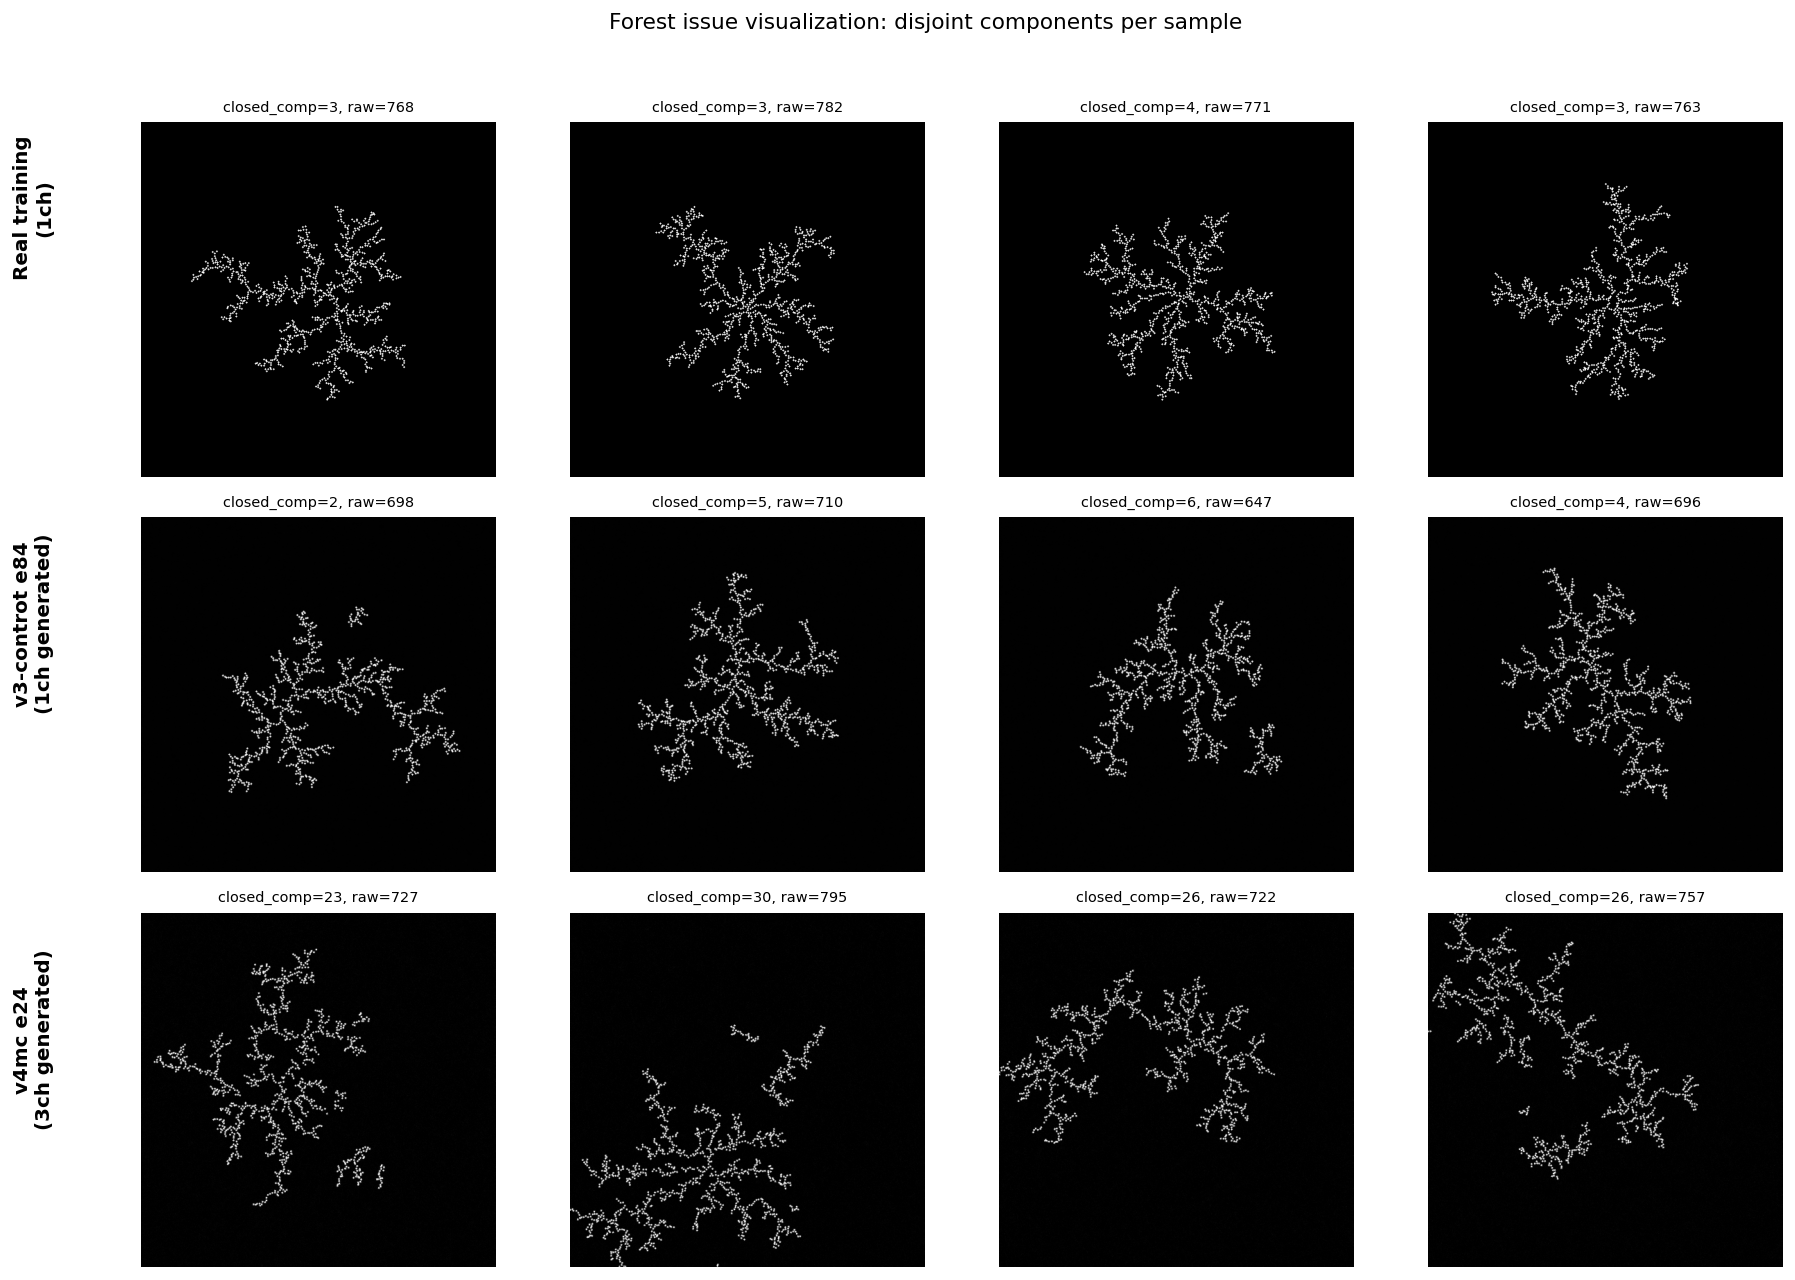
\includegraphics[width=0.92\textwidth]{figures/forest_visual_comparison.png}
\caption{Forest issue: each cell shows one full $512 \times 512$ sample with annotated closed-component and raw-component counts. Top row: real training DLAs render with $2$--$4$ closed components on average due to the $1$-pixel-disc, scale-$2$ render setting. Middle row: \texttt{v3-controt} samples carry $5$--$10$ closed components. Bottom row: \texttt{v4mc} samples carry $15$--$35$, with hundreds of stray single-pixel activations scattered around the main cluster.}
\label{fig:forest_visual}
\end{figure}

The multi-channel pipeline accelerates convergence but exacerbates the forest behavior. Three plausible causes are present: (i) the denoising trajectory has $3\times$ the channels to coordinate, so any partial inconsistency in late steps produces stray activations the binary mask alone would have masked; (ii) there is no explicit cross-channel consistency loss to penalize emissions where, for example, channel-1 has nonzero order but channel-0 has zero presence; (iii) the multi-channel approach allocates supervision uniformly across the cluster but provides no special structural status to the seed, leaving the model free to fragment large clusters into smaller subclusters that each look locally reasonable. We address this in the next experiment.

\subsection{RGB seed-aware encoding with cross-channel consistency}

The fifth model (\texttt{v5}) was trained from scratch on a re-rendered version of the dataset that uses an RGB encoding designed to give the seed a structurally distinct status, paired with a cross-channel consistency loss that directly targets the forest problem.

\textbf{RGB seed-blue encoding.} The seed pixel disc is rendered as $(R, G, B) = (0, 0, 255)$, pure blue. Every other particle is rendered as $(255 d / d_{\max}, 255 d / d_{\max}, 0)$ where $d$ is its Euclidean distance from the seed. Particles satisfy $R = G$ by construction. The seed pixel is the only location in the image where $B$ exceeds threshold. Background is $(0, 0, 0)$. Figure~\ref{fig:rgb_encoding} shows the encoding on three representative training samples.

\begin{figure}[H]
\centering
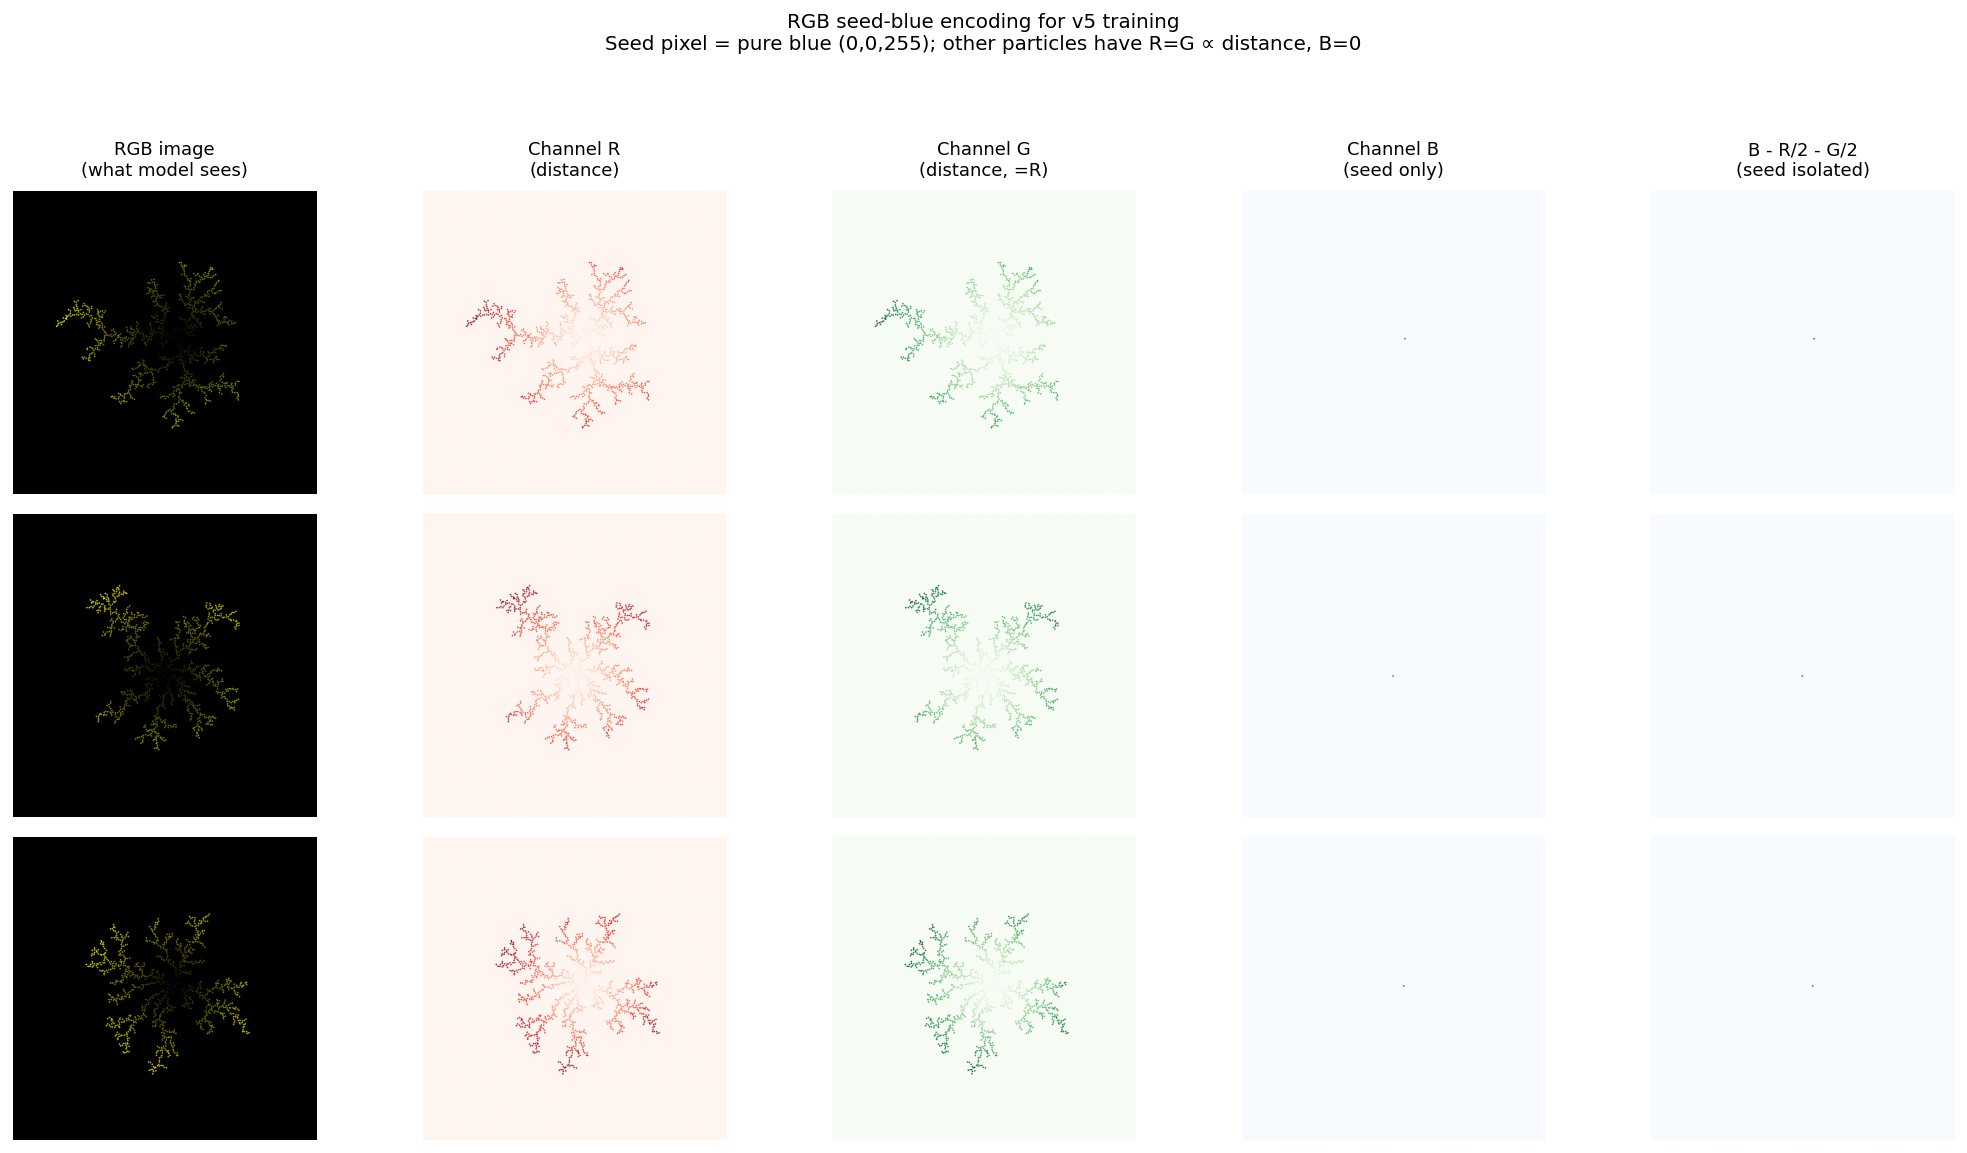
\includegraphics[width=0.95\textwidth]{figures/rgb_encoding_explainer.png}
\caption{RGB seed-aware encoding for the \texttt{v5} pipeline. Five views per sample: composite RGB, R channel alone, G channel alone, B channel alone, and a difference channel $B - R/2 - G/2$ that visually isolates the seed.}
\label{fig:rgb_encoding}
\end{figure}

\textbf{Cross-channel consistency loss.} We add an auxiliary term to the training objective that penalizes physically impossible channel combinations on the predicted $x_0$ recovered from the model's $v$-prediction. The term has two components:
\begin{equation}
\mathcal{L}_{\text{consistency}} = \bigl\langle (R - G)^2 (1 - B)^2 \bigr\rangle + 0.5 \cdot \langle B \cdot R \cdot G \rangle.
\end{equation}
The first part penalizes any pixel where $R \neq G$ except where $B$ is high; this enforces the data constraint that non-seed particles satisfy $R = G$. The second part penalizes coexistence of strong $B$ with strong $R$ or $G$, since the seed disc has $R = G = 0$ and non-seed particles have $B = 0$. We deliberately exclude a sparsity term because legitimate close-to-seed particles have low $R = G$ values by construction.

The total training loss is $\mathcal{L}_{\text{total}} = \mathcal{L}_{\text{diffusion}} + 0.1 \cdot \mathcal{L}_{\text{consistency}}$.

\textbf{Results at epoch 84.} The \texttt{v5} model trained for $84$ epochs to a final training loss of $0.0030$. This is the lowest fully-trained loss of any model in the study: \texttt{v3} plateaued at $0.0035$ across its full $64$-epoch run, \texttt{v3-controt} sat at $0.0057$ at epoch $84$, and \texttt{v4mc} reached $0.0028$ at epoch $24$ but was not trained further. The per-epoch cost of \texttt{v5} was approximately the same as \texttt{v4mc} despite the additional consistency-loss computation, since the auxiliary term reuses the model's $v$-prediction and adds only a handful of pointwise multiplications.

The evaluation at $n = 100$ generated samples versus the same $100$-sample training subset used for the other models reveals a markedly different output distribution. The azimuthal Fourier modes collapse: dipole power $p_1$ drops to $6.0\%$ of training ($0.00026$ vs $0.0043$, KS $p = 4 \times 10^{-35}$) and quadrupole $p_2$ drops to $3.8\%$ of training ($0.0047$ vs $0.124$, $p = 5 \times 10^{-43}$). The mean per-sample dipole magnitude is $|c_1|/N = 0.0016$, $5.1\%$ of the training mean of $0.0324$. The Rayleigh phase test remains uniform on both populations ($p = 0.464$ for generated, $p = 0.41$ for training), as expected. By the azimuthal diagnostics that motivated this entire cycle, \texttt{v5} overshoots training in the direction of greater isotropy.

The connected-component picture is even more dramatic. \texttt{v5} produces samples that are single-connected after the standard closing post-processing in $99\%$ of cases, versus $13\%$ for training and $0\%$ for \texttt{v4mc} at epoch $24$. Mean closed-component count is $1.13$ for \texttt{v5} versus $3.17$ for training. The forest problem identified in Section~4.6 effectively disappears at the closed-component level.

These wins come paired with two new costs that are visible in the raw output. First, the raw pixel-level component count for \texttt{v5} is $13{,}368 \pm 10{,}507$ versus training's $776 \pm 14$. The stray-component count (raw components smaller than $5$ pixels) is $10{,}615 \pm 8{,}690$ versus zero in training. The model emits a sparse low-amplitude pixel-noise floor everywhere in the image; nearly all of those isolated pixels then merge into the central cluster under the closing operation, which is what produces the single-connected result. Second, the raw radius of gyration is $205.5$ versus training's $95.6$, a $2.15\times$ inflation, largely driven by that noise floor at large radius from the COM. Standard post-processing (closing plus largest-component extraction) brings the R$_g$ back down by removing the sparse pixels, but the headline ``before post-processing'' numbers are misleading.

The interpretation we arrived at is that the cross-channel consistency loss does exactly what its mathematics says it does. The $(R - G)^2 (1 - B)^2$ term is zero whenever $R = G$ regardless of the magnitude. A pixel that satisfies $R = G = 0.01$ is just as compliant with the loss as one that satisfies $R = G = 0.7$. The model learns to keep the consistency loss small everywhere by spreading low-amplitude $R = G$ activity over the whole image, which costs nothing under the consistency term and pays a small price under the standard reconstruction loss. The net effect is that the cluster structure is correct (single connected component, isotropic by every angular metric) but the model has invented a pixel-noise floor that is invisible to the consistency loss because it satisfies $R = G$ trivially.

This is, on balance, the most successful encoding of the four. The forest issue is essentially solved, the dipole and quadrupole are both below training rather than above, and the convergence remains fast. The raw-pixel noise floor and the inflated raw $R_g$ are post-processing problems rather than fundamental learning problems, and they are amenable to the same closing-and-largest-component pipeline that \texttt{v3} already uses.

\section{Discussion}

\subsection{What we now know about the failure modes}

The picture that emerged this cycle is that the previous study's diagnosis (``the model learns visual texture rather than DLA dynamics'') is correct at a coarse level but obscures a finer decomposition of the failure into three orthogonal modes.

\textit{Mode 1: directional symmetry leakage.} An augmentation pipeline that samples from the wrong symmetry group leaks into the learned distribution. The $D_4$ bug was real and the patch worked exactly as expected: it closed the topology and angular-variance gaps. This is purely a data-pipeline issue with a known fix.

\textit{Mode 2: missing structural prior on topology.} The forest analysis shows that single-channel models, even at the bulk-stat saturation point, produce more disjoint pieces than training. The multi-channel encoding's order channel makes loops actively expensive and the model learns this early in training. This is a representation issue addressed by enriching the input.

\textit{Mode 3: per-sample geometric variance.} The dipole magnitude inflation is not fixed by either of the above. Per-sample lopsidedness is a property of the generated cluster's mass distribution around its own COM, in random directions, and neither rotation augmentation nor structural channels affect it. The RGB encoding's cross-channel consistency loss attacks this mode indirectly by giving the model a stricter set of admissible local patterns, but the data shows the dipole gap closes only modestly under that change. More direct attacks (auxiliary loss on $|c_1|$, larger model, longer training) remain open.

The decomposition matters because it suggests that targeted interventions will close targeted gaps. Last cycle's framing was that diffusion models cannot learn DLA dynamics from images. The current framing is that they can learn some properties (bulk statistics, topology under the right encoding, isotropy of the ensemble) and not others (per-sample geometric variance), and that the failures are diagnosable.

\subsection{Cost of the multi-channel approach}

The convergence speedup from \texttt{v4mc} is real, but the multi-channel model takes more memory and exhibits worse forest behavior during training. Both effects scale with the channel count. The RGB encoding used in \texttt{v5} keeps the channel count at $3$ but redistributes the information so that the seed is structurally distinct rather than just an extreme value of two auxiliary fields. The cross-channel consistency loss eliminates the forest problem at the closed-component level (single-connected fraction climbs from $0\%$ in \texttt{v4mc} to $99\%$ in \texttt{v5}, well above the $13\%$ baseline that the training images themselves achieve at this render setting) but introduces a sparse pixel-noise floor that inflates raw component counts. The noise floor is a consequence of the consistency-loss geometry: any $R = G$ pattern at any amplitude satisfies the constraint, so the model has no gradient pressure to drive low-amplitude pixels to zero. A future iteration of the loss should include an explicit suppression term that activates only below an amplitude threshold; the current implementation deliberately omitted such a term to avoid penalizing legitimate close-to-seed particles, but a threshold-gated version could discriminate the two cases.

\subsection{What we did not do this cycle}

We did not implement particle-count conditioning, fractal-dimension box-counting on the new samples, or skeletonization-based post-processing integration with the main evaluation pipeline. The mass-radius scaling needed to estimate $D_f$ would also benefit from a multi-$N$ dataset; both are planned for the next cycle. We did not run a 1024-resolution attempt; the bumped-resolution attempt from the previous cycle is still pending GPU availability and a stable multi-channel encoding.

\section{Future Directions}

\textbf{Auxiliary loss on per-sample $|c_1|$ with careful Goodhart mitigation.} The dipole magnitude has resisted augmentation, structural encoding, and cross-channel consistency fixes alike. A direct penalty during training is the obvious next move; the principal risk is that the model learns to satisfy the metric without internalizing the underlying isotropy. A reasonable design is to train two models in parallel, one with the auxiliary loss and one without, and confirm that the model with the loss also matches the broader spectrum (modes $k = 3$ onward), not just $k = 1$.

\textbf{Skeletonization-based post-processing.} The current closing-based post-processing fixes the largest-component count but does not enforce strict tree topology. A skeletonization stage that extracts the medial axis and then breaks any remaining cycles at their weakest edge would produce strict trees by construction. The infrastructure is already partially in place in \texttt{eval/skeleton\_samples.py}.

\textbf{Higher resolution and conditioning.} Both items are carried from previous cycles. The multi-channel approach's lower compute cost per training epoch makes 1024-resolution more feasible than it was last cycle. Particle-count conditioning (passing the target $N$ as a scalar to the denoiser) would let us measure mass-radius scaling without needing a separate dataset per $N$.

\textbf{Skeleton-conditioned cascaded diffusion.} The most ambitious option is to factor generation into two stages: a small model that produces a skeleton (a thin, structurally clean tree) followed by a renderer model that thickens the skeleton into pixel-space output. Each stage is a simpler problem than the joint one and topology is enforced at the skeleton stage by construction.

\section{Conclusion}

The headline result this cycle is that a custom-built DDPM with $v$-prediction and a controlled training pipeline reaches bulk-statistic agreement with the training distribution, and that the residual gap revealed by finer diagnostics decomposes into three separable failure modes. The augmentation bug is fixed by sampling continuous rotations and resolves the directional component. The multi-channel encoding produces a $7\times$ convergence speedup and resolves the topology gap once given enough training. The RGB seed-blue encoding paired with a cross-channel consistency loss reaches the lowest fully-trained loss of any model in the study ($0.0030$ at epoch $84$), drives the dipole and quadrupole power fractions to roughly $6\%$ and $4\%$ of training respectively, and produces single-connected output in $99\%$ of generated samples versus the $13\%$ rate of the training images themselves. The same encoding introduces a pixel-noise floor that inflates raw component counts and raw radius of gyration; standard closing-plus-largest-component post-processing removes most of this noise. Per-sample dipole magnitude inflation, which persisted across the first three model variants, is the failure mode that the cross-channel consistency loss actually closes; what remains is a calibration problem (the model now produces samples that are slightly \emph{more} isotropic than training) rather than the inflation we started the cycle worried about. The full progression takes the work from bulk statistics matching last cycle, through a diagnosable decomposition of failure modes, to an architecture that produces samples whose structural metrics fall below training on the dimensions the diagnostics were designed to measure.

\section*{Acknowledgments}

This work was conducted under the supervision of Jonathan Machta at the University of Massachusetts Amherst. Compute resources were provided by the UMass Amherst Unity HPC cluster. We thank the lucidrains group for the open-source \texttt{denoising-diffusion-pytorch} implementation that served as the architectural reference for our custom DDPM, and the maintainers of \texttt{scipy} and \texttt{matplotlib} which the entire evaluation suite depends on.

\begin{thebibliography}{99}

\bibitem{desouza2026learning}
V.\ DeSouza and J.\ Machta. Learning Physical Aggregation: Diffusion-Limited Aggregation via Diffusion Models. Technical Report, UMass Amherst, January 2026.

\bibitem{wittensander1981}
T.\ A.\ Witten and L.\ M.\ Sander. Diffusion-Limited Aggregation, a Kinetic Critical Phenomenon. \textit{Phys.\ Rev.\ Lett.}, 47(19):1400--1403, 1981.

\bibitem{meakin1998}
P.\ Meakin. \textit{Fractals, Scaling and Growth Far from Equilibrium}. Cambridge University Press, 1998.

\bibitem{machta2013}
J.\ Machta. Natural complexity, computational complexity, and depth. \textit{Chaos}, 23(3):037111, 2013.

\bibitem{ho2020ddpm}
J.\ Ho, A.\ Jain, and P.\ Abbeel. Denoising Diffusion Probabilistic Models. \textit{NeurIPS}, 33:6840--6851, 2020.

\bibitem{salimans2022progressive}
T.\ Salimans and J.\ Ho. Progressive Distillation for Fast Sampling of Diffusion Models. \textit{ICLR}, 2022.

\bibitem{hang2023efficient}
T.\ Hang, S.\ Gu, C.\ Li, J.\ Bao, D.\ Chen, H.\ Hu, X.\ Geng, and B.\ Guo. Efficient Diffusion Training via Min-SNR Weighting Strategy. \textit{ICCV}, 2023.

\bibitem{nichol2021improved}
A.\ Nichol and P.\ Dhariwal. Improved Denoising Diffusion Probabilistic Models. \textit{ICML}, 2021.

\bibitem{song2020ddim}
J.\ Song, C.\ Meng, and S.\ Ermon. Denoising Diffusion Implicit Models. \textit{ICLR}, 2021.

\bibitem{ronneberger2015unet}
O.\ Ronneberger, P.\ Fischer, and T.\ Brox. U-Net: Convolutional Networks for Biomedical Image Segmentation. \textit{MICCAI}, 2015.

\bibitem{rombach2022ldm}
R.\ Rombach, A.\ Blattmann, D.\ Lorenz, P.\ Esser, and B.\ Ommer. High-Resolution Image Synthesis with Latent Diffusion Models. \textit{CVPR}, 2022.

\bibitem{sohl2015nonequilibrium}
J.\ Sohl-Dickstein, E.\ Weiss, N.\ Maheswaranathan, and S.\ Ganguli. Deep Unsupervised Learning using Nonequilibrium Thermodynamics. \textit{ICML}, 2015.

\bibitem{karras2022elucidating}
T.\ Karras, M.\ Aittala, T.\ Aila, and S.\ Laine. Elucidating the Design Space of Diffusion-Based Generative Models. \textit{NeurIPS}, 2022.

\bibitem{fisher1995statistical}
N.\ I.\ Fisher. \textit{Statistical Analysis of Circular Data}. Cambridge University Press, 1995.

\bibitem{massey1951ks}
F.\ J.\ Massey. The Kolmogorov-Smirnov Test for Goodness of Fit. \textit{Journal of the American Statistical Association}, 46(253):68--78, 1951.

\bibitem{lucidrains2024ddpm}
P.\ Wang. \texttt{denoising-diffusion-pytorch}. GitHub repository, 2020--present. \\
\url{https://github.com/lucidrains/denoising-diffusion-pytorch}

\bibitem{harris2020array}
C.\ R.\ Harris et al. Array programming with NumPy. \textit{Nature}, 585:357--362, 2020.

\bibitem{virtanen2020scipy}
P.\ Virtanen et al. SciPy 1.0: fundamental algorithms for scientific computing in Python. \textit{Nature Methods}, 17:261--272, 2020.

\bibitem{paszke2019pytorch}
A.\ Paszke et al. PyTorch: An Imperative Style, High-Performance Deep Learning Library. \textit{NeurIPS}, 32, 2019.

\end{thebibliography}

\end{document}
